\subsection{Recommender systems}

\begin{frame}{Recommender systems}
    \begin{itemize}
        \item Help consumers by providing suggestions that are expected to satisfy
            their tastes.
    \end{itemize}
    \begin{center}
        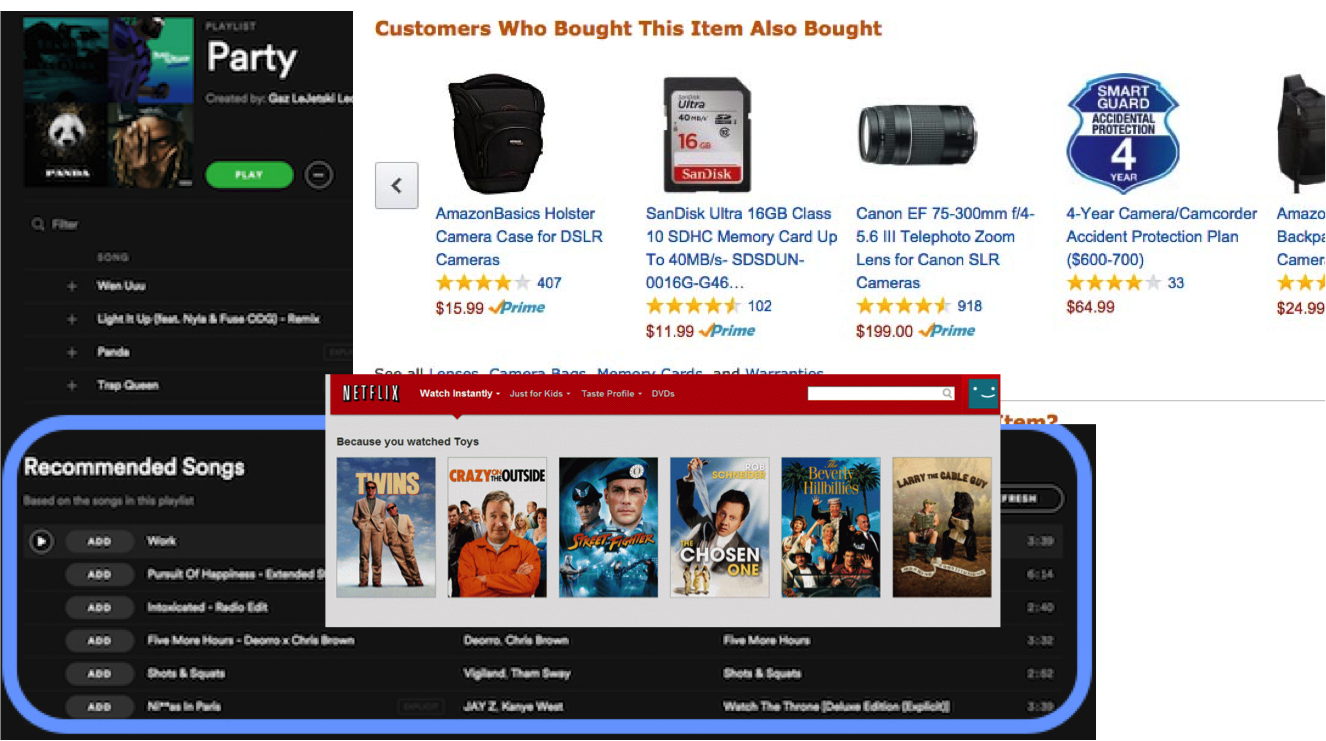
\includegraphics[scale=0.5]{recsys}
    \end{center}
\end{frame}


\begin{frame}{Methods}
    \begin{itemize}
        \item Non-personalized 
            \begin{itemize}
                \item Models that rely on global properties, e.g., item popularity.
            \end{itemize}
        \item Content-based
            \begin{itemize}
                \item Models that use the similarity between a user's profile and a item attributes. 
            \end{itemize}
        \item Collaborative filtering-based
            \begin{itemize}
                \item Models that rely on similarities among the users or the items.
            \end{itemize}
    \end{itemize}
\end{frame}


\begin{frame}{Collaborative filtering methods}
    \begin{itemize}
        \item Use the user preferences available over the items, e.g., ratings (explicit) or like/dislike (implicit). 

        \item Neighborhood-based : Learn the user or the item neighborhood based on the co-rating information, e.g., UserKNN~\footcite{herlocker1999algorithmic}, ItemKNN~\footcite{SarwarKarypis01}, SLIM~\footcite{r0}.

        \item Matrix completion-based : Learn an explicit model from the user preferences, e.g., MF~\footcite{Koren2009}, BPRMF~\footcite{rendle2009bpr}.

    \end{itemize}
    %TODO: include image of user-item rating matrices
\end{frame}



